
\section{关键性质的定义与证明}

本节完全可以留待很久之后再读；我们将要用到的那些事实都已在上一节中陈述过了。不过，这些论证并不复杂，所以你不妨立刻就读。阅读时，你应当回过头去，把上一节中的那些事实逐条核对打钩，好让自己确信：所许诺的一切，你都懂得了。

\textbf{18.2.1. \trCechCohomology{}（Čech cohomology）。}\quad 一般框架下的\trCechCohomology{}是用对一空间越来越细的覆盖取极限来定义的。而在我们的代数几何框架中，情形要干净得多：我们可以只用单个覆盖。

设 $X$ \trQuasicompact{}且\trSeparated——例如当 $X$ 在 $A$ 上\trQuasiprojective{}时即如此。特别地，$X$ 可被有限多个\trAffine{}开集覆盖，且任意两个\trAffine{}开集之交仍是一个\trAffine{}开集（由\trSeparatedness，\mbox{命题~11.2.13}）。我们之所以使用\trQuasicompactness{}与\trSeparatedness，只是为了保证这两条好性质。

设 $\mathscr{F}$ 是一个\trQCSheaf，而 $\mathscr{U}=\{\mathfrak{U}_i\}_{i=1}^{n}$ 是由覆盖 $X$ 的\trAffine{}开集组成的一个\emph{有限}族。对 $I\subset\{1,\dots,n\}$，定义 $\mathfrak{U}_I=\bigcap_{i\in I}\mathfrak{U}_i$，由分离假设，它是\trAffine{}的。（对那些在其他背景下见过\trCohomology{}的读者，这里有一个极强的类比：用有限多个开集 $\mathfrak{U}_i$ 覆盖一个\trTopologicalSpace{} $X$，使得一切交 $\bigcap_{i\in I}\mathfrak{U}_i$ 都\trContractible。）考虑\textbf{\trCech\trComplexN}（Čech complex）
\begin{equation*}\tag{18.2.1.1}\label{eq:cech-complex}
\begin{aligned}
0\longrightarrow\prod_{\substack{|I|=1\\ I\subset\{1,\dots,n\}}}\mathscr{F}(\mathfrak{U}_I)\longrightarrow\cdots\longrightarrow{}\\
\prod_{\substack{|I|=i\\ I\subset\{1,\dots,n\}}}\mathscr{F}(\mathfrak{U}_I)\longrightarrow\prod_{\substack{|I|=i+1\\ I\subset\{1,\dots,n\}}}\mathscr{F}(\mathfrak{U}_I)\longrightarrow\cdots.
\end{aligned}
\end{equation*}

诸映射定义如下。除非 $I\subset J$（也就是说 $J=I\cup\{j\}$），否则从 $\mathscr{F}(\mathfrak{U}_I)\to\mathscr{F}(\mathfrak{U}_J)$ 的映射是 $0$。若 $j$ 是 $J$ 的第 $k$ 个元素，则该映射便是限制映射 $\mathrm{res}_{\mathfrak{U}_I,\mathfrak{U}_J}$ 的 $(-1)^{k-1}$ 倍。

\textbf{18.2.A.（容易的练习：致那些从未见过类似\trCech\trComplexN{}之物的读者）}\quad 证明：\trCech\trComplexN{}确实是一个\trComplexN，也就是说，相邻两支箭头的复合是 $0$。

定义 $\mathrm{H}^i_{\mathscr{U}}(X,\mathscr{F})$ 为复形 \eqref{eq:cech-complex} 的第 $i$ 个\trCohomology{}群。（指标从 $i=0$ 起算。）注意，若 $X$ 是一个 $A$-\trScheme，则 $\mathrm{H}^i_{\mathscr{U}}(X,\mathscr{F})$ 是一个 $A$-\trModule。我们差不多就要成功地定义出\trCechCohomology{}群 $\mathrm{H}^i$ 了，只可惜我们的定义先验地依赖于覆盖 $\mathscr{U}$ 的选取。注意，$\mathrm{H}^i_{\mathscr{U}}(X,\cdot)$ 显然是一个\trCovariantFunctor{} $\mathit{QCoh}_X\to\mathit{Mod}_A$。

\textbf{18.2.B.（容易的练习）}\quad 把 $\mathrm{H}^0_{\mathscr{U}}(X,\mathscr{F})$ 与 $\Gamma(X,\mathscr{F})$ 等同起来。（提示：使用 $\mathscr{F}$ 的\trSheaf{}公理。）

\textbf{18.2.C.（练习）}\quad 设
\begin{equation*}\tag{18.2.1.2}\label{eq:ses-sheaves-topological}
0\longrightarrow\mathscr{F}\longrightarrow\mathscr{G}\longrightarrow\mathscr{H}\longrightarrow 0
\end{equation*}
是一个\trTopologicalSpace{}上诸\trAbelianGroups{}层的\trShortExactSequence，而 $\mathscr{U}$ 是一个有限开覆盖，使得对 $\mathscr{U}$ 中诸开子集的任意交 $\mathfrak{U}_I$，映射 $\Gamma(\mathfrak{U}_I,\mathscr{G})\to\Gamma(\mathfrak{U}_I,\mathscr{H})$ 都是满射。证明：我们得到「$\mathrm{H}^i_{\mathscr{U}}$ 的\trCohomology{}\trLongExactSequence」（其中我们对 $\mathrm{H}^i_{\mathscr{U}}$ 采用同样的定义）。在我们的情形——$X$ 是一个\trQuasicompact\trSeparated{}的 $A$-\trScheme，而 \eqref{eq:ses-sheaves-topological} 是 $X$ 上诸\trQCSheaf{}的\trShortExactSequence——证明：我们得到 $A$-\trModule{} $\mathrm{H}^i_{\mathscr{U}}$ 的一个\trLongExactSequence。

在\mbox{定理~18.2.4}与\mbox{定理~18.7.1}的证明中，我们将用到你的连接同态构造所具有的一个特点：它将「与 $A$ 的局部化交换」。更精确地说，我们将需要下面这条练习。

\textbf{18.2.D.（练习）}\quad 设在\trQuasicompact\trSeparated{}的 $A$-\trScheme{} $\pi\colon X\to\Spec A$ 上给定诸\trQCSheaf{}的一个\trShortExactSequence{} \eqref{eq:ses-sheaves-topological}、由\trAffine{}开集组成的 $X$ 的一个覆盖 $\mathscr{U}$、以及某个 $f\in A$。把 $\mathscr{U}$ 的诸开集限制到 $X_f$ 上，便给出 $X_f=\pi^{-1}(\mathrm{D}(f))$ 的一个\trAffine{}开覆盖 $\mathscr{U}'$。请把「用 $\mathrm{H}^i_{\mathscr{U}}$ 并在 $f$ 处局部化而得到的、与 \eqref{eq:ses-sheaves-topological} 相伴的\trLongExactSequence」等同于「用\trAffine{}开覆盖 $\mathscr{U}'$ 而得到的、与 \eqref{eq:ses-sheaves-topological} 限制到 $X_f$ 上者相伴的\trLongExactSequence」。（先检验由协变性给出的那些映射——例如 $\mathrm{H}^i_{\mathscr{U}}(\mathscr{F})\to\mathrm{H}^i_{\mathscr{U}}(\mathscr{G})$——都「与局部化交换」，然后检验连接同态也如此。）

\textbf{18.2.2.\ \trhTheorem{}/\trhDefinition{。}}\ ——\ \emph{我们的\trStandingHypothesis{}是：$X$ \trQuasicompact{}且\trSeparated。$\mathrm{H}^i_{\mathscr{U}}(X,\mathscr{F})$ 不依赖于（有限）覆盖 $\{\mathfrak{U}_i\}$ 的选取。更精确地说，对任意两个覆盖 $\{\mathfrak{U}_i\}\subset\{V_i\}$，由\trCech\trComplexN{} \eqref{eq:cech-complex} 的自然映射所诱导的诸映射 $\mathrm{H}^i_{\{V_i\}}(X,\mathscr{F})\to\mathrm{H}^i_{\{\mathfrak{U}_i\}}(X,\mathscr{F})$ 都是\trIsomorphism。定义\textbf{\trCechCohomology{}群} $\mathrm{H}^i(X,\mathscr{F})$ 为这个群。}

如果你还不清楚「\trCech\trComplexN{}的自然映射」指的是什么，那么见到 \eqref{eq:les-complexes} 时它自会明朗。

\textbf{18.2.3.}\quad 致专家：在\trCohomology{}群上诱导出\trIsomorphism{}的那些复形间的映射称作\textbf{\trQuasiisomorphism}（quasiisomorphism）。由这个构造我们实际得到的，其实是比\trCohomology{}更细的不变量：我们得到的是 $A$-模的\emph{\trDerivedCategory}（derived category）中的一个元素。

\emph{证明。}\quad 只需在 $|\{V_i\}|=|\{\mathfrak{U}_i\}|+1$ 的情形证明该结果。我们将证明：若 $\{\mathfrak{U}_i\}_{1\le i\le n}$ 是 $X$ 的一个覆盖，而 $\mathfrak{U}_0$ 是任意另外一个\trAffine{}开集，则映射 $\mathrm{H}^i_{\{\mathfrak{U}_i\}_{0\le i\le n}}(X,\mathscr{F})\to\mathrm{H}^i_{\{\mathfrak{U}_i\}_{1\le i\le n}}(X,\mathscr{F})$ 是一个\trIsomorphism。考虑复形的如下\trExactSequence
\begin{equation*}\tag{18.2.3.1}\label{eq:les-complexes}
\begin{tikzcd}[row sep=2.9em, column sep=1.6em]
& 0 \ar[d] & 0 \ar[d] & 0 \ar[d] & \\
\cdots \ar[r] & \prod\limits_{\substack{|I|=i-1\\ 0\in I}}\mathscr{F}(\mathfrak{U}_I) \ar[r] \ar[d] & \prod\limits_{\substack{|I|=i\\ 0\in I}}\mathscr{F}(\mathfrak{U}_I) \ar[r] \ar[d] & \prod\limits_{\substack{|I|=i+1\\ 0\in I}}\mathscr{F}(\mathfrak{U}_I) \ar[r] \ar[d] & \cdots \\
\cdots \ar[r] & \prod\limits_{|I|=i-1}\mathscr{F}(\mathfrak{U}_I) \ar[r] \ar[d] & \prod\limits_{|I|=i}\mathscr{F}(\mathfrak{U}_I) \ar[r] \ar[d] & \prod\limits_{|I|=i+1}\mathscr{F}(\mathfrak{U}_I) \ar[r] \ar[d] & \cdots \\
\cdots \ar[r] & \prod\limits_{\substack{|I|=i-1\\ 0\notin I}}\mathscr{F}(\mathfrak{U}_I) \ar[r] \ar[d] & \prod\limits_{\substack{|I|=i\\ 0\notin I}}\mathscr{F}(\mathfrak{U}_I) \ar[r] \ar[d] & \prod\limits_{\substack{|I|=i+1\\ 0\notin I}}\mathscr{F}(\mathfrak{U}_I) \ar[r] \ar[d] & \cdots \\
& 0 & 0 & 0. &
\end{tikzcd}
\end{equation*}

通篇约定 $I\subset\{0,\dots,n\}$。下面两行是关于两个覆盖的\trCech\trComplexN，而二者之间的映射诱导出我们所想要的那个\trCohomology{}上的映射。从这个复形的\trShortExactSequence{}我们得到\trCohomology{}的\trLongExactSequence（\mbox{定理~1.5.8}）。于是我们希望证明顶行正合，从而其\trCohomology{}消失。（注意 $\mathfrak{U}_0\cap\mathfrak{U}_j$ 由我们的分离假设是\trAffine{}的，\mbox{命题~11.2.13}。）但顶行的第 $i$ 个\trCohomology{}恰恰是 $\mathrm{H}^{i-1}_{\{\mathfrak{U}_j\cap\mathfrak{U}_0\}_{j>0}}(\mathfrak{U}_0,\mathscr{F})$，唯独在起点处例外，那里我们得到 $0$（因为这个复形从 $0\to\mathscr{F}(\mathfrak{U}_0)\to\prod_{j=1}^{n}\mathscr{F}(\mathfrak{U}_0\cap\mathfrak{U}_j)$ 出发）。所以，只需证明仿射概形的更高次\trCech{}群是 $0$。于是由下述结果，证明即告完成。\hfill$\square$

\textbf{18.2.4.\ \trhTheorem{。}}\ ——\ \emph{\trAffine{} $A$-\trScheme{} $X$ 的更高次\trCechCohomology{} $\mathrm{H}^i_{\mathscr{U}}(X,\mathscr{F})$ 消失（对任意\trAffine{}覆盖 $\mathscr{U}$、$i>0$ 与\trQCSheaf{} $\mathscr{F}$）。}

这是又一次「\trPartitionOfUnity」式的论证，其精神与\mbox{定理~4.1.2}的证明如出一辙。

\emph{证明。}\quad 我们想证明「扩充」复形
\begin{equation*}\tag{18.2.4.1}\label{eq:extended-cech-complex}
0\longrightarrow\mathscr{F}(X)\longrightarrow\prod_{|I|=1}\mathscr{F}(\mathfrak{U}_I)\longrightarrow\prod_{|I|=2}\mathscr{F}(\mathfrak{U}_I)\longrightarrow\cdots
\end{equation*}
（即在开头添上了\trGlobalSections{} $\mathscr{F}(X)$）没有\trCohomology，也就是说，是正合的。（顺带一提，这个扩充复形称作 $\mathscr{F}(X)$ 的\textbf{\trCech{}分解}（Čech resolution），这里是相对于覆盖 $\mathscr{U}$ 的这一选取而言。）我们用一个技巧来做到这一点。

先设某个 $\mathfrak{U}_i$（比如说 $\mathfrak{U}_0$）就是 $X$。我们用障眼法来处理这种情形。\eqref{eq:extended-cech-complex} 这个复形正是下面这列复形的\trShortExactSequence{}的中间一行：
\begin{equation*}\tag{18.2.4.2}\label{eq:sleight-short-exact}
\begin{tikzcd}[row sep=3.4em, column sep=2em]
0 \ar[r] & 0 \ar[r] \ar[d] & \prod\limits_{|I|=1,0\in I}\mathscr{F}(\mathfrak{U}_I) \ar[r] \ar[d] & \prod\limits_{|I|=2,0\in I}\mathscr{F}(\mathfrak{U}_I) \ar[r] \ar[d] & \cdots \\
0 \ar[r] & \mathscr{F}(X) \ar[r] \ar[d] & \prod\limits_{|I|=1}\mathscr{F}(\mathfrak{U}_I) \ar[r] \ar[d] & \prod\limits_{|I|=2}\mathscr{F}(\mathfrak{U}_I) \ar[r] \ar[d] & \cdots \\
0 \ar[r] & \mathscr{F}(X) \ar[r] & \prod\limits_{|I|=1,0\notin I}\mathscr{F}(\mathfrak{U}_I) \ar[r] & \prod\limits_{|I|=2,0\notin I}\mathscr{F}(\mathfrak{U}_I) \ar[r] & \cdots
\end{tikzcd}
\end{equation*}
顶行就是底行向左平移一格的结果。相应的\trCohomology{}\trLongExactSequence{}表明，中间一行的\trCohomology{}消失。（你应当自行证明\trCohomology{}上的「连接同态」确实是一个\trIsomorphism。）这或许会让你想起\trMappingCone{}构造（\mbox{练习~1.6.E}）。（这里还有一个技巧，能从另一个角度达成这一段的目标。设 $\mathrm{id}$ 是复形 \eqref{eq:extended-cech-complex} 与其自身之间的恒等映射，又设 $0$ 是复形 \eqref{eq:extended-cech-complex} 与其自身之间的零映射。请描述 $\mathrm{id}$ 与 $0$ 之间的一个显式\trHomotopy；参 \S1.5.7。这个\trHomotopy{}将用到与 \eqref{eq:les-complexes} 相同的「想法」。于是，\trHomology{}上的恒等映射便等于\trHomology{}上的零映射（\mbox{练习~1.5.E}），故\trHomology{}必为零。这个想法颇有启发性，因为它还会在其他场合被用到。）

\begin{figure}[htbp]
\centering
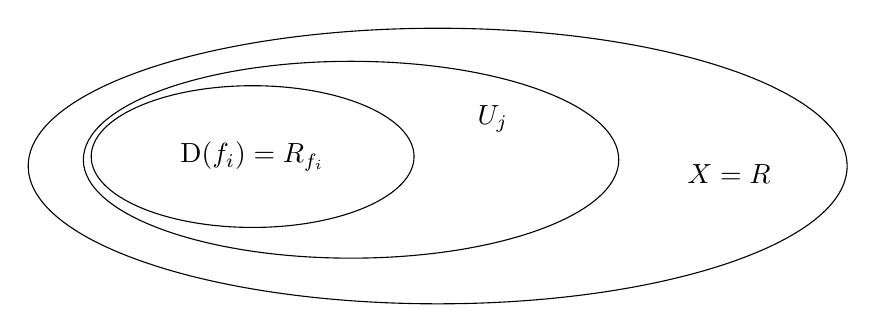
\begin{tikzpicture}[line join=round]
\draw (0,0) ellipse (5.2 and 1.75);
\draw (-1.1,0.08) ellipse (3.4 and 1.25);
\draw (-2.35,0.12) ellipse (2.05 and 0.9);
\node at (-2.35,0.12) {$\mathrm{D}(f_i)=\Spec R_{f_i}$};
\node at (0.7,0.6) {$\mathfrak{U}_j$};
\node at (3.7,-0.1) {$X=\Spec R$};
\end{tikzpicture}
\caption{\mbox{定理~18.2.2} 证明的最后一步。（依原书手绘图重绘。）}\label{fig:cech-final-step}
\end{figure}

最后，我们用再一记障眼法证明一般情形。设 $X=\Spec R$。我们想证明 $A$-模复形 \eqref{eq:extended-cech-complex} 是正合的。它同时也是 $R$-模的复形，于是我们想证明 $R$-模复形 \eqref{eq:extended-cech-complex} 是正合的。为证其正合，只需证明：对 $\Spec R$ 的由特异开集 $\mathrm{D}(f_i)$（$1\le i\le r$）组成的一个覆盖（也就是说 $(f_1,\dots,f_r)=1$ 于 $R$ 中），该复形是正合的。（翻译一下：层的序列的正合性可以局部检验。）我们如此选取覆盖，使得每个 $\mathrm{D}(f_i)$ 都含于我们的某个\trAffine{}开子集 $\mathfrak{U}_j$ 之中（见图~\ref{fig:cech-final-step}）。把复形 \eqref{eq:extended-cech-complex} 在 $f_i$ 处局部化，便得到 $\mathrm{D}(f_i)$ 关于其\trAffine{}覆盖 $\{\mathfrak{U}_k\cap\mathrm{D}(f_i)\}$ 的\trCech\trComplexN。我们要证明这个复形（对固定的 $i$ 与 $j$）是正合的。但这正是上一段处理过的情形——诸\trAffine{}开集之一，$\mathfrak{U}_j\cap\mathrm{D}(f_i)$，就等于 $\mathrm{D}(f_i)$。\hfill$\square$

至此，我们已证明了前一节的性质 \textbf{(i)--(iii)}。「仿射覆盖上同调消失」这条性质 \textbf{(vi)} 也同样直截了当：若 $X$ 被 $n$ 个\trAffine{}开集覆盖，就拿这些开集来充当覆盖 $\mathscr{U}$，并注意到\trCech\trComplexN{}在第 $n$ 步就终结了。

\textbf{18.2.E.（练习：性质 (v)）}\quad 设 $\pi\colon X\to Y$ 是一个\trAffine\trMorphism，$Y$ 是一个\trQuasicompact{}且\trSeparated{}的 $A$-\trScheme（从而 $X$ 亦是如此，因为\trAffine{}\trMorphism{}既\trQuasicompact{}又\trSeparated）。若 $\mathscr{F}$ 是 $X$ 上的一个\trQCSheaf，请描述一个自然的\trIsomorphism
$\mathrm{H}^i(Y,\pi_*\mathscr{F})\overset{\sim}{\longleftarrow}\mathrm{H}^i(X,\mathscr{F})$。（提示：若 $\mathscr{U}$ 是 $Y$ 的一个\trAffine{}覆盖，则「$\pi^{-1}(\mathscr{U})$」就是 $X$ 的一个\trAffine{}覆盖。用这两个覆盖来计算 $\mathscr{F}$ 的\trCohomology。）

\textbf{18.2.F.（练习：性质 (iv)）}\quad 设 $\pi\colon X\to Y$ 是任意一个\trQuasicompact\trSeparated{}\trMorphism，$\mathscr{F}$ 是 $X$ 上的一个\trQCSheaf，而 $Y$ 是一个\trQuasicompact\trSeparated{}的 $A$-\trScheme。对 $\pi$ 的这些假设保证 $\pi_*\mathscr{F}$ 是 $Y$ 上的一个\trQCSheaf。请描述一个自然的态射 $\mathrm{H}^i(Y,\pi_*\mathscr{F})\to\mathrm{H}^i(X,\mathscr{F})$，它是 $\Gamma(Y,\pi_*\mathscr{F})\to\Gamma(X,\mathscr{F})$ 的扩充。（旁注：这个态射在 $i=0$ 时是\trIsomorphism，但在更高的 $i$ 处未必是：考虑 $i=1$、$X=\mathbb{P}^1_k$、$\mathscr{F}=\OO(-2)$，而取 $Y$ 为一点 $\Spec k$。）

\textbf{18.2.G.（练习）}\quad 证明前一节的性质 \textbf{(vii)}，即「\trCohomology{}与\trFiltered\trColimit{}交换」。（这件事可以徒手完成。提示：在环上模的范畴中，对一个滤过集们取余极限是一个正合函子，\S1.5.14。）\footnote{原书此处作「taking the colimit over a filtered sets」，语法不通，疑当为「over a filtered set」之误，兹照录原书。——译者注}

至此，前一节的性质我们已尽数证毕，唯有 \textbf{(viii)} 除外，它将在 \S18.3 中处理。

\textbf{18.2.5. $k$-\trScheme{}上关于\trCohomology{}的若干有用事实。}

\textbf{18.2.H.（练习：\trCohomology{}与基域的变换）}\quad 设 $X$ 是一个\trQuasicompact\trSeparated{}的 $k$-\trScheme，$\mathscr{F}$ 是 $X$ 上的一个\trQCSheaf。给出一个对一切 $i$ 成立的\trIsomorphism
\[
\mathrm{H}^i(X,\mathscr{F})\otimes_k K\overset{\sim}{\longleftarrow}\mathrm{H}^i(X\times_{\Spec k}\Spec K,\mathscr{F}\otimes_k K)
\]
其中 $K/k$ 是任意一个\trFieldExtension。这里 $\mathscr{F}\otimes_k K$ 指的是 $\mathscr{F}$ 拉回到 $X\times_{\Spec k}\Spec K$ 上的结果。于是 $h^i(X,\mathscr{F})=h^i(X\times_{\Spec k}\Spec K,\mathscr{F}\otimes_k K)$。（这条同构对「把关于 $k$-\trScheme{}的事实过渡为关于代数闭域上概形的事实」很有用。你的证明或许会以一种根本的方式用到\trVectorSpace{}——也就是说，线性代数。若果真没用到，那么，当 $k\to K$ 被换成一个平坦\trRingMorphism{} $B\to A$ 时，你仍可以证明一个更一般的结论。回忆一下：$B\to A$ 称作平坦的，若 $\otimes_B A$ 是一个正合函子 $\mathit{Mod}_B\to\mathit{Mod}_A$。给这条更难的练习一个提示：\mbox{FHHF 定理}，\mbox{练习~1.5.I}。至于下一步的推广，见\mbox{练习~18.7.B(b)}。）

\textbf{18.2.I.（练习：无基点性与基域扩张无关）}\quad 设 $X$ 是一个\trQuasicompact\trSeparated{}的 $k$-\trScheme，$\mathscr{L}$ 是 $X$ 上的一个\trInvertibleSheaf，而 $K/k$ 是一个\trFieldExtension。证明：$\mathscr{L}$ 是\trBasePointFree{}的，当且仅当它拉回到 $X\times_{\Spec k}\Spec K$ 上是\trBasePointFree{}的。（提示：取 $i=0$ 的\mbox{练习~18.2.H}表明：$\mathscr{L}$ 在 $k$ 上的诸\trSection{}的一个基，在与 $K$ 作张量之后，便成为 $\mathscr{L}\otimes_k K$ 的诸\trSection{}的一个基。）

\textbf{18.2.6.\ \trhTheorem{}（射影 $k$-\trScheme{}上诸\trQCSheaf{}的维数\trCohomology{}消失）。}\ ——\ \emph{设 $X$ 是一个\trProjective{} $k$-\trScheme，$\mathscr{F}$ 是 $X$ 上的一个\trQCSheaf。则当 $i>\dim X$ 时，$\mathrm{H}^i(X,\mathscr{F})=0$。}

换言之，\trCohomology{}在高于 $X$ 之\trDimension{}的一切次数上都消失。

\emph{证明。}\quad 设 $X\hookrightarrow\mathbb{P}^N$，并令 $n=\dim X$。我们来证明 $X$ 可以被 $n+1$ 个\trAffine{}开集覆盖。\mbox{练习~12.3.D} 表明：$\mathbb{P}^N$ 上存在 $n+1$ 个\trEffectiveCartierDivisor，使得它们的\trComplement{} $\mathfrak{U}_0,\dots,\mathfrak{U}_n$ 覆盖 $X$。于是 $\mathfrak{U}_i$ 是\trAffine{}的，从而 $\mathfrak{U}_i\cap X$ 是\trAffine{}的，这样我们便用 $n+1$ 个\trAffine{}开集覆盖了 $X$。\hfill$\square$

（事实证明，$n+1$ 个\trAffine{}开集总是必需的。证明这一点的途径之一，是证明稠密\trAffine{}开子集的\trComplement{}总是纯余维数 $1$ 的；例如见 [RotV, Lem.~2.3]。）

\textbf{18.2.7.}\ \hard\ \textbf{更一般情形的维数\trCohomology{}消失。}\quad 借助\trBlowup{}的理论，\mbox{定理~18.2.6} 可以被推广到拟射影 $k$-\trScheme；见 \S22.4.15。维数\trCohomology{}消失甚至在一般得多的框架下也成立。为了陈述它，我们需要用\trDerivedFunctor{}（第 23 章）这套更一般的机器来定义\trCohomology。若 $X$ 是一个\trNoetherian\trTopologicalSpace（\S3.6.14），而 $\mathscr{F}$ 是 $X$ 上任意一个阿贝尔群的层，则对一切 $i>\dim X$ 都有 $\mathrm{H}^i(X,\mathscr{F})=0$。（\trGrothendieck{}在 [GrS, pp.~29--30] 中勾勒了他那优雅的证明；更详细的讲解见 [Ha1, Theorem~III.2.7]。）特别地，若 $X$ 是一个\trDimension{}为 $n$ 的 $k$-\trVariety，则我们\emph{总是}有维数\trCohomology{}消失，甚至对那些疯狂到无法用 $n+1$ 个\trAffine{}开子集覆盖的簇也是如此（见 \S22.4.15）。
